\chapter{Significado F\'isico del Par\'ametro \( q \) de Tsallis}\label{ch-PhysicalMeaningQ}

\fancyhf{} % clear all header fields
\fancyhead[LE]{\nouppercase{\textbf{Cap\'itulo 5. Significado f\'isico del \\par\'ametro \( q \) \hfill\emph{\rightmark}}}}
\fancyhead[RO]{\nouppercase{\emph{\rightmark}\hfill\textbf{Cap\'itulo 5. Significado f\'isico del \\par\'ametro \( q \)}}}
\fancyfoot[LE]{\nouppercase{\thepage\hfill {Pressure Distribution Inside Nucleons in a Tsallis-MIT Bag Model}}}
\fancyfoot[RO]{\nouppercase{{Pressure Distribution Inside Nucleons in a Tsallis-MIT Bag Model} \hfill \thepage}}

\begin{chaptersummary}
Este cap\'itulo analiza el significado f\'isico del par\'ametro de no extensividad \( q \) en el contexto del modelo de bolsa. Se argumenta que \( q \) encapsula de manera natural la f\'isica del confinamiento de quarks y gluones, eliminando la necesidad expl\'icita de introducir una presi\'on de bolsa fija \( B \). As\'i, se establece una relaci\'on entre \( q \) y \( B \), sugiriendo una reinterpretaci\'on del confinamiento en t\'erminos de correlaciones estad\'isticas no extensivas.
\end{chaptersummary}

\section{Confinamiento y Presi\'on de Bolsa}
En el modelo de bolsa tradicional, los quarks est\'an confinados dentro de una regi\'on espacial debido a una presi\'on de vac\'io \( B \) que evita su escape. La densidad Lagrangiana correspondiente se expresa como:

\begin{equation}
{L}_{\mathrm{bag}} = \left( {L}_{\mathrm{QCD}} - B \right) \theta_V
\end{equation}

donde \( \theta_V \) es la funci\'on escal\'on de Heaviside que define el interior de la bolsa.

\section{Interpretaci\'on Alternativa mediante \( q \)}
La presi\'on de bolsa \( B \) es un par\'ametro fenomenol\'ogico que modela la energ\'ia de las fluctuaciones del vac\'io QCD. Sin embargo, al considerar correlaciones estad\'isticas no extensivas, el par\'ametro \( q \) puede reinterpretarse como una medida de dichas correlaciones, evitando la necesidad de introducir un \( B \) expl\'icito.

\break

\section{Relaci\'on entre \( q \) y la Presi\'on de Bolsa}
Bajo esta perspectiva, la presi\'on total en el modelo de bolsa puede reescribirse como:

\begin{equation}
P_q(T,\mu) = P_{q_0}(T,\mu) - B(r)
\end{equation}

o alternativamente, aislando \( q \):

\begin{equation}
q(r) = q_0 + \frac{B(r)}{\dfrac{256 \pi^2}{15} \left( \dfrac{\pi^2}{90} + \dfrac{1}{30} \left( \dfrac{\mu}{T} \right)^2 \right) V T^7}
\label{eq:q-bag-relation}
\end{equation}

donde \( V \) es el volumen efectivo de la bolsa y \( (T, \mu) \) representan la temperatura y potencial qu\'imico locales.

\section{Implicaciones F\'isicas}
Esta relaci\'on implica que el confinamiento puede interpretarse como una consecuencia natural de las correlaciones entre part\'iculas en un sistema fuertemente acoplado, caracterizado por \( q > 1 \). En consecuencia, el modelo estad\'istico de Tsallis proporciona una descripci\'on m\'as fundamental del confinamiento en t\'erminos de la termodin\'amica de sistemas no extensivos.

\section{Dependencia radial del par\'ametro \( q \)}

La expresi\'on~\eqref{eq:q-bag-relation} no solo sugiere una equivalencia formal entre \( q \) y \( B \), sino que establece una relaci\'on funcional expl\'icita entre el par\'ametro de Tsallis y el radio:

\[
q(r) = q_0 + \frac{B(r)}{C(T,\mu)}
\quad \text{con} \quad
C(T,\mu) = \frac{256 \pi^2}{15} \left( \frac{\pi^2}{90} + \frac{1}{30} \left( \frac{\mu}{T(r)} \right)^2 \right) V T(r)^7
\]

donde \( T(r) \) y \( B(r) \) son perfiles radiales obtenidos en el Cap\'itulo~\ref{ch-ProtonBagParameters}, y \( q_0 \) corresponde al valor de referencia sin presi\'on de bolsa.

\begin{remark}[Interpretaci\'on din\'amica]
    Esta formulaci\'on implica que el confinamiento no es un efecto est\'atico, sino una propiedad emergente local que var\'ia con el radio. En particular, \( q(r) \) crece en las regiones donde la presi\'on de bolsa es mayor, como en la periferia del prot\'on, capturando as\'i el car\'acter no homog\'eneo del confinamiento.
\end{remark}

\section{Visualización y análisis de la relación \( q \leftrightarrow B \)}

Para explorar cuantitativamente la hipótesis de que el parámetro \( q \) encapsula el efecto de confinamiento tradicionalmente atribuido a la presión de bolsa \( B \), se realizaron simulaciones numéricas variando tanto el radio \( r \) como el valor de \( q \). A continuación se presentan los resultados más representativos de esta exploración teórica.

\begin{figure}[H]
    \centering
    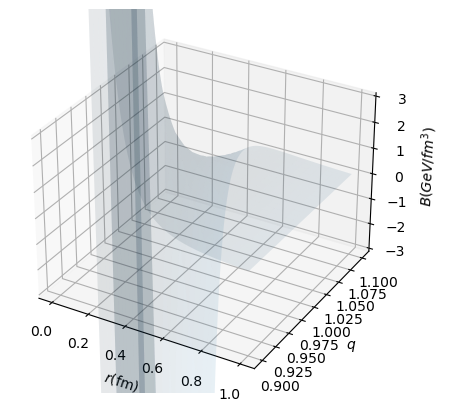
\includegraphics[width=0.5\textwidth]{./Images/B_vs_q_vs_r.png}
    \caption[Superficie \( B(q, r) \)]{Superficie tridimensional que muestra la presión de bolsa \( B \) en función de \( q \) y el radio \( r \), obtenida a partir de la expresión inversa discutida en la ecuación~\eqref{eq:q-bag-relation} (con $\mu = 0$). Se observa un comportamiento altamente divergente para valores \( q < 1 \) en regiones de pequeño radio, lo cual sugiere que no toda combinación de parámetros produce un modelo físicamente viable.}
    \label{fig:B_vs_q_vs_r}
\end{figure}

\begin{figure}[H]
    \centering
    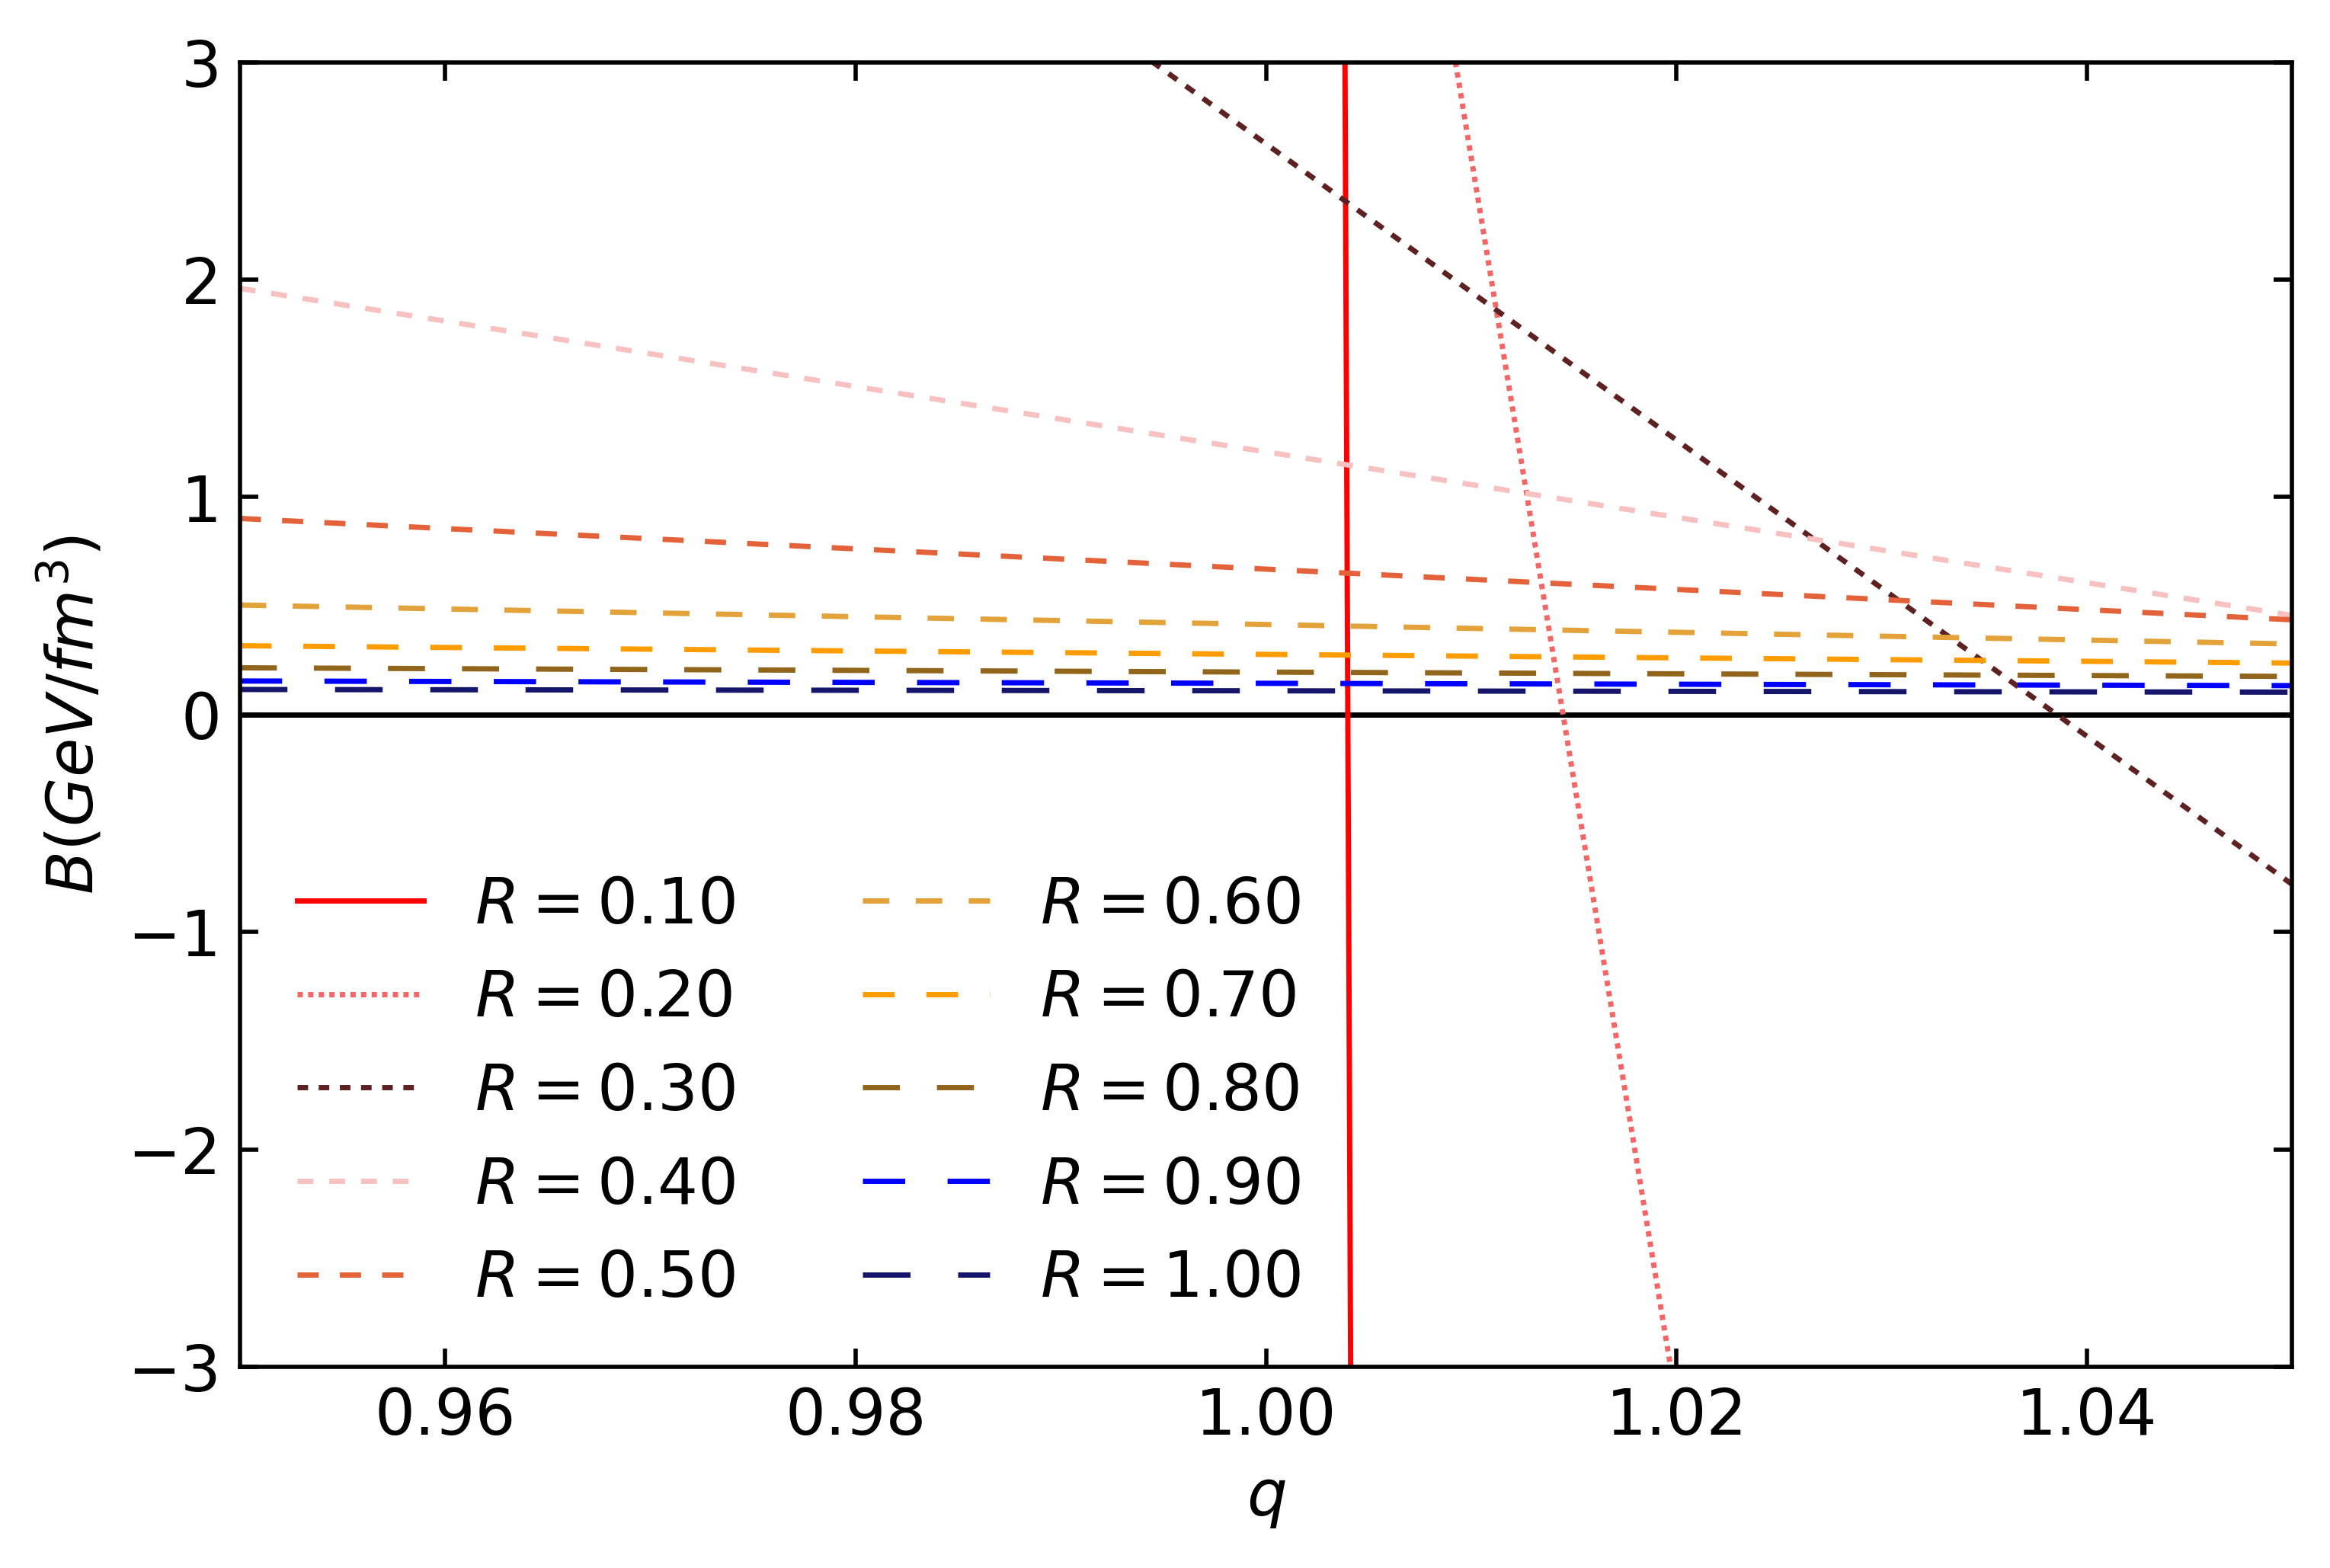
\includegraphics[width=0.85\textwidth]{./Images/BvsQcuts.png}
    \caption[Cortes radiales de \( B \) en función de \( q \)]{Relación lineal entre la presión de bolsa \( B \) y el parámetro de Tsallis \( q \), para diferentes valores fijos de \( r \). 
Cada curva corresponde a una función lineal de la forma \( B(q) = a(r)(1.002 - q) + b(r) \), donde los coeficientes dependen del radio. 
Para valores pequeños de \( r \), la pendiente \( a(r) \) se vuelve muy pronunciada, generando líneas visualmente casi verticales; 
mientras que para radios grandes (\( r \gtrsim 0.6\,\text{fm} \)), las pendientes disminuyen y las curvas se aplanan. 
Este comportamiento es coherente con los cortes esperados de la superficie \( B(q, r) \) presentada en la figura tridimensional \ref{fig:B_vs_q_vs_r}.
}
    \label{fig:BvsQcuts}
\end{figure}

\begin{remark}[Delimitación física del dominio]
    Estas gráficas indican que no cualquier valor de \( q \) resulta físicamente válido para un radio dado. Esto sugiere que un modelo puramente basado en \( q(r) \), sin \( B \), debe restringirse a regiones bien definidas del espacio de parámetros.
\end{remark}

Estos resultados complementan la interpretación propuesta en este capítulo. Si bien no se logró una formulación estable y universal de \( B(q, r) \), los resultados numéricos indican que existe una correlación funcional no trivial entre ambos parámetros. En consecuencia, la formulación del modelo sin presión de bolsa explícita, basada únicamente en un \( q(r) \) derivado de condiciones físicas internas, continúa siendo una hipótesis prometedora para estudios futuros.

\section{Reconstrucci\'on de \( B(r) \) para diferentes valores de \( q \)}

Para verificar la consistencia del modelo con la idea de que \( q \) puede absorber el efecto de \( B \), se explor\'o la posibilidad inversa: reconstruir \( B(r) \) a partir de un valor conocido de \( q \). En la siguiente figura se comparan dos perfiles de presi\'on efectiva obtenidos con diferentes formas funcionales de \( B(r) \), asociadas a distintos valores de \( q \).

\begin{figure}[H]
    \centering
    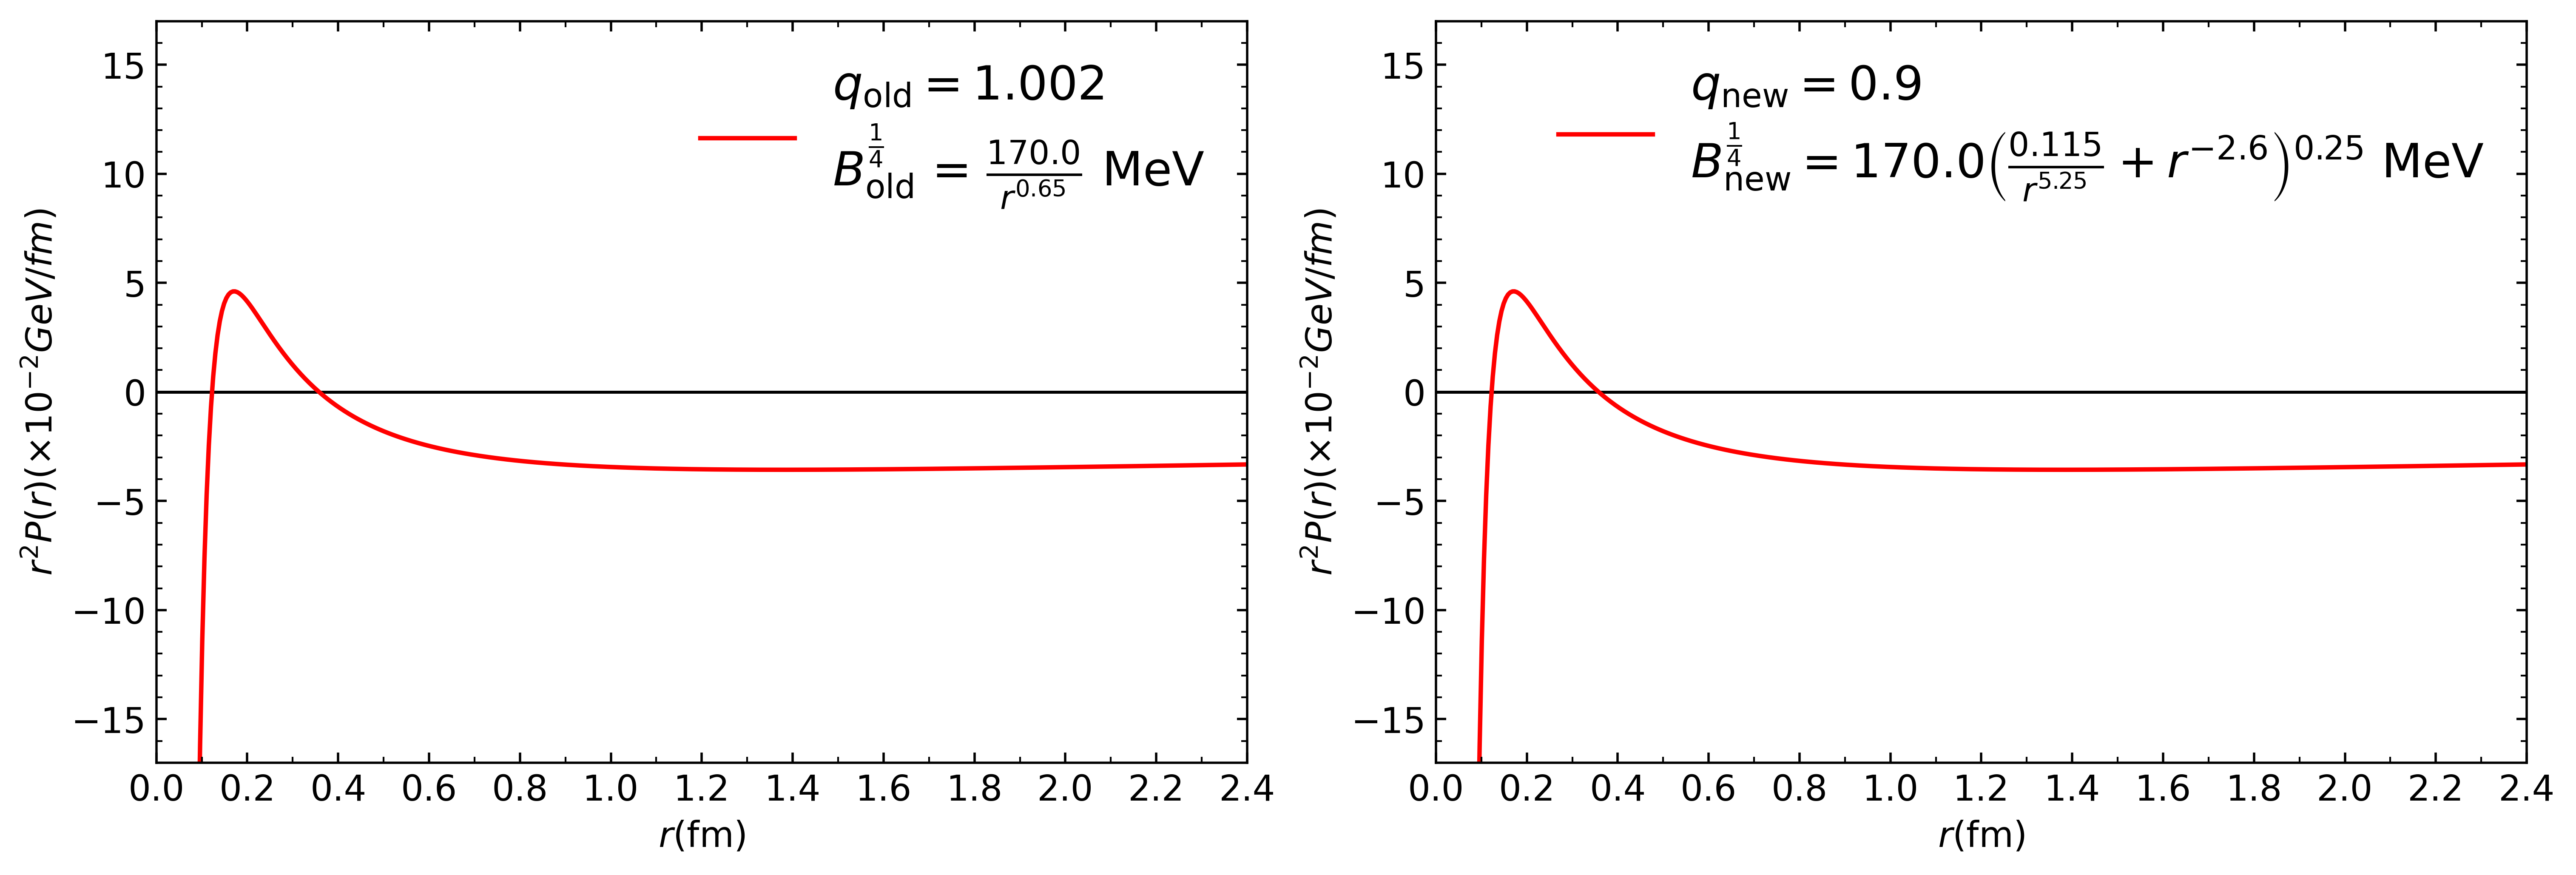
\includegraphics[width=0.95\textwidth]{./Images/Comparacion_B_old_new_dual.png}
    \caption[Reconstrucci\'on de \( B(r) \) para diferentes \( q \)]{Reconstrucci\'on de la presi\'on de bolsa a partir de dos valores distintos del par\'ametro de Tsallis. \textbf{Izquierda:} Forma tradicional \( B^{1/4}(r) = 170\,r^{-0.65} \,\mathrm{MeV} \) correspondiente a \( q = 1.002 \). \textbf{Derecha:} Forma alternativa ajustada para \( q = 0.9 \), que resulta en una presi\'on radial similar, pero sin requerir \( B(r) \) expl\'icita.}
    \label{fig:B_reconstructed_dual}
\end{figure}

\begin{figure}[H]
    \centering
    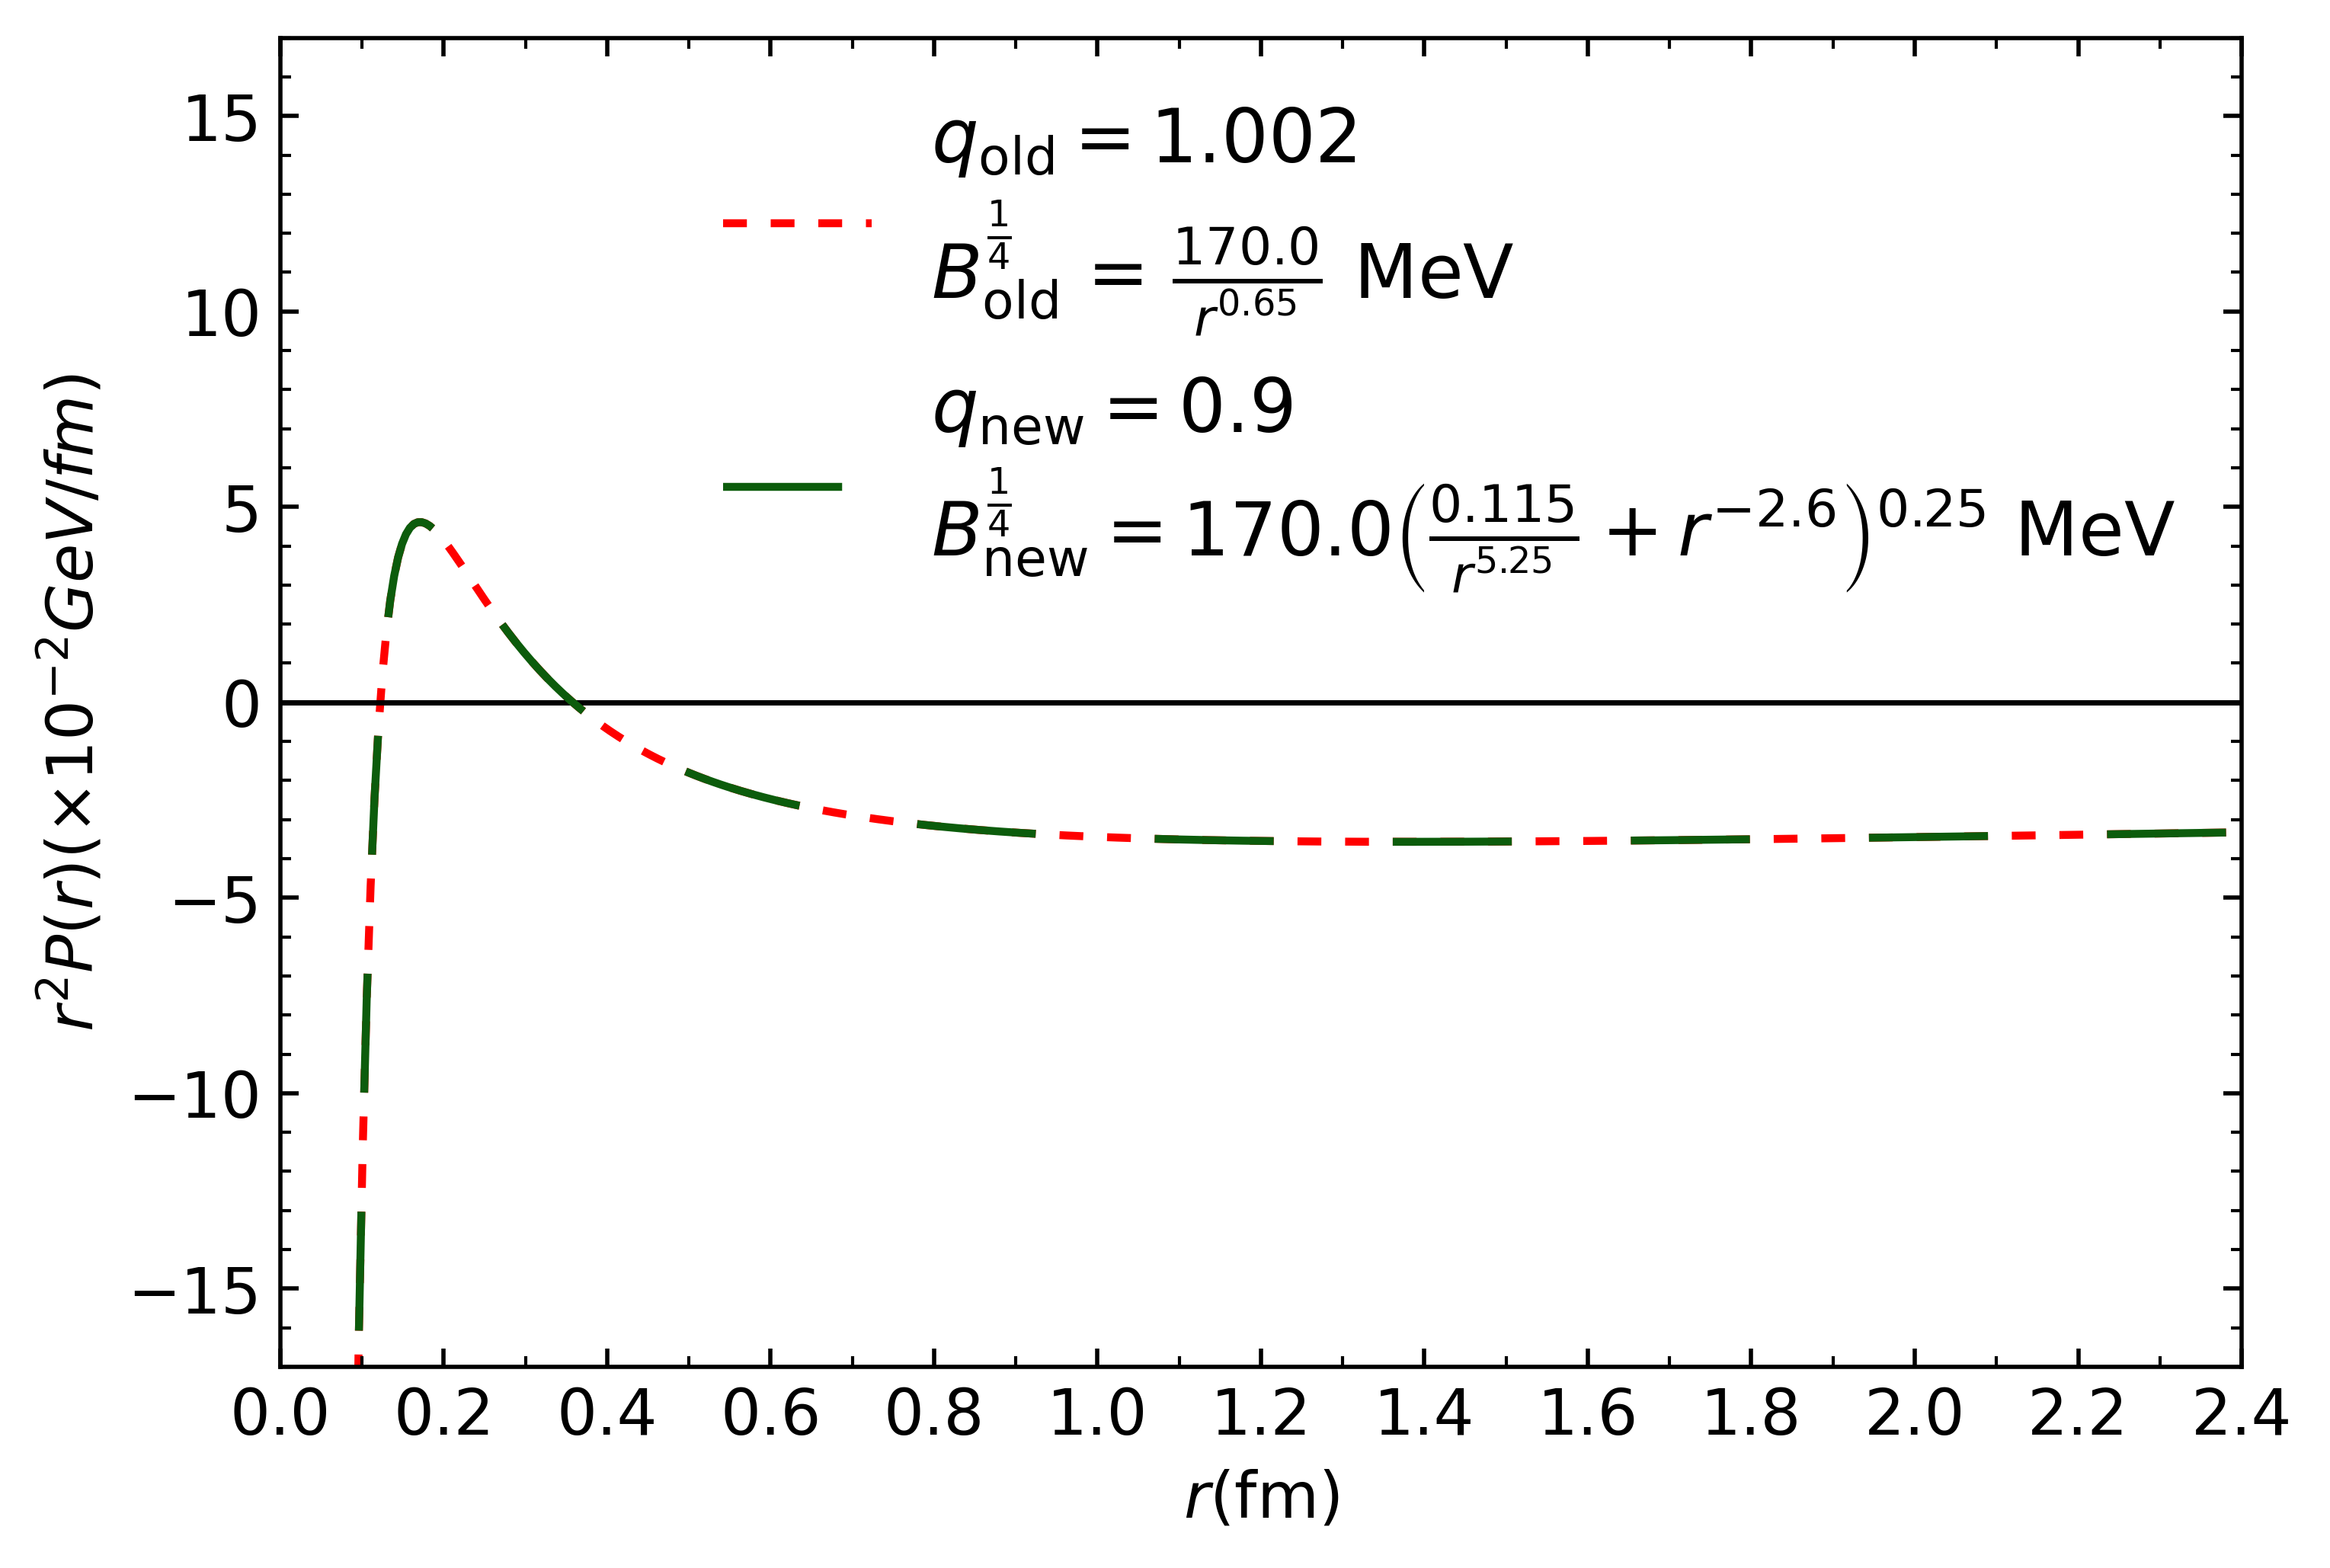
\includegraphics[width=0.75\textwidth]{./Images/Comparacion_B_old_new_combined.png}
    \caption[Comparaci\'on entre presiones con \( q = 1.002 \) y \( q = 0.9 \)]{Comparaci\'on directa entre las distribuciones de presi\'on ponderada \( r^2 P(r) \) utilizando dos formas distintas de \( B^{1/4}(r) \): una tradicional (rojo) y otra reconstruida a partir de un valor m\'as bajo de \( q \) (verde). Se observa que ambos enfoques conducen a perfiles similares de presi\'on efectiva, reforzando la hip\'otesis de que \( q \) puede sustituir el papel de \( B \) bajo ciertas condiciones.}
    \label{fig:B_reconstructed_combined}
\end{figure}
\begin{remark}[Exploración adicional sobre energía de Tsallis]
    Como parte del análisis conceptual del confinamiento, se exploró una posible relación entre la masa total del hadrón\cite{Johnson1975} y la energía interna de un sistema descrito por la estadística de Tsallis. A partir de relaciones de Maxwell y la formulación termodinámica no extensiva, se propuso una energía total del sistema de la forma:
    
    \[
    U_q(T, V) = F_q(T, V) + T S_q(T, V) = \frac{37 \pi^2}{30} V T^4 + \frac{128 \pi^4}{225} (1 - q) V^2 T^7
    \]
    
    donde \( F_q \) y \( S_q \) corresponden respectivamente a la energía libre de Helmholtz y a la entropía en el marco de Tsallis, y los factores numéricos provienen del conteo de grados de libertad en el gas de quarks y gluones.
    
    Se intentó igualar esta energía a la masa del hadrón obtenida mediante el modelo de bolsa estándar (\( M_{\text{bag}} \approx U_q \)), con el fin de despejar el valor del parámetro \( q \) en función del volumen y temperatura locales. Sin embargo, como los parámetros \( V \) y \( T \) ya estaban determinados por la geometría y condiciones térmicas del modelo, el procedimiento condujo a un despeje trivial de \( q \), sin contenido predictivo.
    
    Aunque esta vía no produjo un resultado cuantitativo relevante, representa un esfuerzo por reinterpretar la energía de confinamiento como una propiedad emergente de correlaciones no extensivas. Su desarrollo completo requeriría una incorporación más rigurosa del formalismo de Tsallis en la cuantización de modos o en la formulación efectiva de las contribuciones energéticas del modelo de bolsa.
\end{remark}

\section*{Conclusi\'on del cap\'itulo}

En este cap\'itulo se ha propuesto una reinterpretaci\'on del par\'ametro de no extensividad \( q \) como un descriptor efectivo del confinamiento en el modelo de bolsa, eliminando la necesidad expl\'icita de una presi\'on de bolsa fija \( B \). A trav\'es de un an\'alisis funcional y exploraciones num\'ericas, se mostr\'o que \( q \) y \( B \) guardan una relaci\'on estructurada dependiente del radio, reflejando propiedades locales del sistema. Aunque el desarrollo de un modelo completamente autoconfinante basado en \( q(r) \) a\'un requiere refinamientos te\'oricos y computacionales, los resultados obtenidos respaldan la hip\'otesis de que el confinamiento puede ser entendido como una manifestaci\'on de correlaciones no extensivas internas. Este enfoque abre nuevas perspectivas para futuras investigaciones en la f\'isica de hadrones y materia fuertemente correlacionada.
